% An open neighborhood U (dashed) of a point x inside a space X (blob).
% Source: book/tex/topology/top-more.tex (§ definition of open neighborhood).
\documentclass[border=2mm]{standalone}
\usepackage{tikz}
\begin{document}
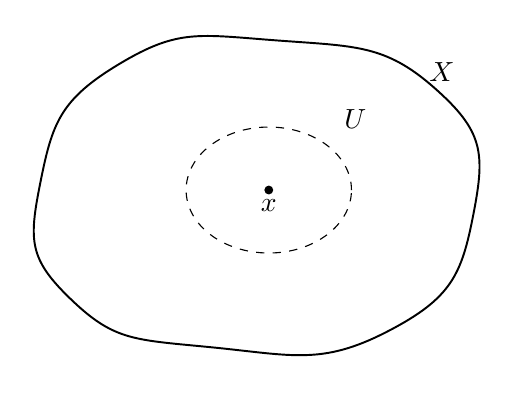
\begin{tikzpicture}[scale=1]
  \draw[black, line width=0.7pt]
    plot[smooth cycle, tension=0.9]
    coordinates {(-2.6,0.2) (-1.6,1.7) (0.4,2.0) (2.4,1.4) (2.9,-0.2)
                 (1.8,-1.7) (-0.4,-1.9) (-2.2,-1.3)};
  \node at (2.5,1.6) {$X$};
  \fill (0.3,0.1) circle (1.6pt) node[below] {$x$};
  \draw[dashed] (0.3,0.1) ellipse (1.05 and 0.8);
  \node at (1.4,1.0) {$U$};
\end{tikzpicture}
\end{document}
